\documentclass{beamer}
\usepackage{tikz,amsmath,hyperref,graphicx,stackrel,animate}
\usetikzlibrary{positioning,shadows,arrows,shapes,calc}
\newcommand{\argmax}{\operatornamewithlimits{argmax}}
\newcommand{\argmin}{\operatornamewithlimits{argmin}}
\mode<presentation>{\usetheme{Frankfurt}}
\AtBeginSection[]
{
  \begin{frame}<beamer>
    \frametitle{Outline}
    \tableofcontents[currentsection,currentsubsection]
  \end{frame}
}
\title{Lecture 9: Convolution}
\author{Mark Hasegawa-Johnson\\These slides are in the public domain.}
\date{ECE 401: Signal and Image Analysis, Fall 2023}  
\begin{document}

% Title
\begin{frame}
  \maketitle
\end{frame}

% Title
\begin{frame}
  \tableofcontents
\end{frame}

%%%%%%%%%%%%%%%%%%%%%%%%%%%%%%%%%%%%%%%%%%%%
\section[Outline]{Outline of today's lecture}
\setcounter{subsection}{1}
\begin{frame}
  \frametitle{Outline of today's lecture}
  \begin{enumerate}
  \item HW3 and MP3
  \item Local averaging
  \item Convolution
  \item Differencing
  \item Edge Detection
  \end{enumerate}
\end{frame}

%%%%%%%%%%%%%%%%%%%%%%%%%%%%%%%%%%%%%%%%%%%%
\section[Averaging]{Local averaging}
\setcounter{subsection}{1}

\begin{frame}
  \frametitle{How do you treat an image as a signal?}
  \centerline{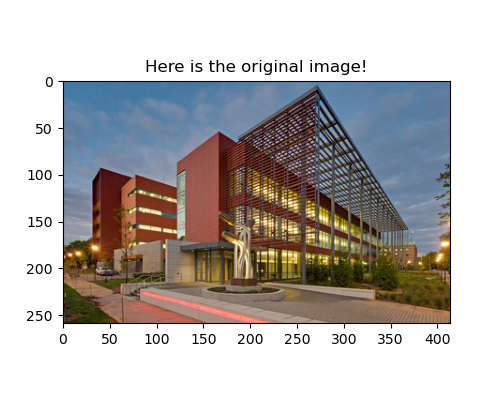
\includegraphics[height=3.5in]{mp3fig1.png}}
\end{frame}

\begin{frame}
  \frametitle{How do you treat an image as a signal?}
  \begin{itemize}
  \item
    An RGB image is a signal in three dimensions: $f[i,j,k]=$
    intensity of the signal in the $i^{\textrm{th}}$ row,
    $j^{\textrm{th}}$ column, and $k^{\textrm{th}}$ color.
  \item
    $f[i,j,k]$, for each $(i,j,k)$, is either stored as an integer or
    a floating point number:
    \begin{itemize}
    \item Floating point: usually $x\in[0,1]$, so $x=0$ means dark,
      $x=1$ means bright.
    \item Integer: usually $x\in\left\{0,\ldots,255\right\}$, so
      $x=0$ means dark, $x=255$ means bright.
    \end{itemize}
  \item The three color planes are usually:
    \begin{itemize}
    \item $k=0$: Red
    \item $k=1$: Blue
    \item $k=2$: Green
    \end{itemize}
  \end{itemize}
\end{frame}
    
\begin{frame}
  \frametitle{Local averaging}
  \centerline{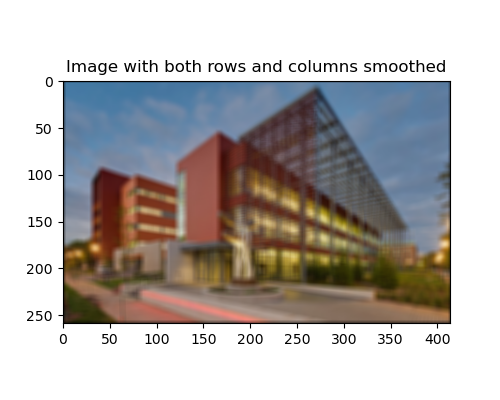
\includegraphics[height=3.5in]{mp3fig4.png}}
\end{frame}

\begin{frame}
  \frametitle{Local averaging}

  \begin{itemize}
    \item 
      ``Local averaging'' means that we create an output image,
      $y[i,j,k]$, each of whose pixels is an {\bf\em average} of nearby
      pixels in $f[i,j,k]$.
    \item
      For example, if we average along the rows:
      \[
      y[i,j,k] = \frac{1}{2M+1}\sum_{j'=j-M}^{j+M} f[i,j',k]
      \]
    \item
      If we average along the columns:
      \[
      y[i,j,k] = \frac{1}{2M+1}\sum_{i'=i-M}^{i+M} f[i',j,k]
      \]
  \end{itemize}
\end{frame}

\begin{frame}
  \frametitle{Local averaging of a unit step}
  The top row are the
  averaging weights.  If it's a 7-sample local average, $(2M+1)=7$, so
  the averaging weights are each $\frac{1}{2M+1}=\frac{1}{7}$.  The
  middle row shows the input, $f[n]$.  The bottom row shows the
  output, $y[n]$.
  \centerline{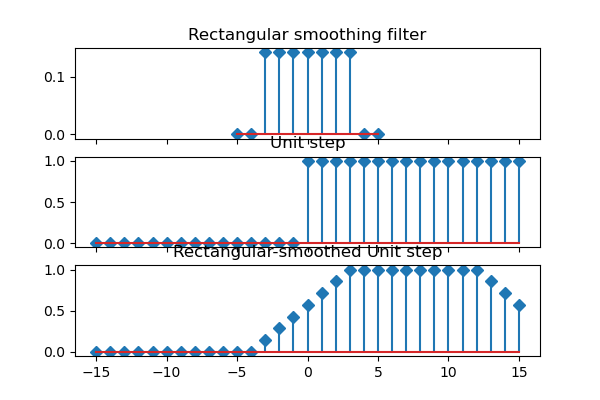
\includegraphics[height=2.5in]{mp3fig2.png}}
\end{frame}

%%%%%%%%%%%%%%%%%%%%%%%%%%%%%%%%%%%%%%%%%%%%
\section[Weighted]{Weighted Local Averaging}
\setcounter{subsection}{1}

\begin{frame}
  \frametitle{Weighted local averaging}

  \begin{itemize}
    \item 
      Suppose we don't want the edges quite so abrupt.  We could do
      that using ``weighted local averaging:'' each pixel of
      $y[i,j,k]$ is a {\bf\em weighted average} of nearby pixels in
      $f[i,j,k]$, with some averaging weights $g[n]$.
    \item
      For example, if we average along the rows:
      \[
      y[i,j,k] = \sum_{m=j-M}^{j+M} g[j-m] f[i,m,k]
      \]
    \item
      If we average along the columns:
      \[
      y[i,j,k] = \sum_{i'=i-M}^{i+M} g[i-m] f[m,j,k]
      \]
  \end{itemize}
\end{frame}

\begin{frame}
  \frametitle{Weighted local averaging of a unit step} The top row are
  the averaging weights, $g[n]$.  The middle row shows the input,
  $f[n]$.  The bottom row shows the output, $y[n]$.
  \centerline{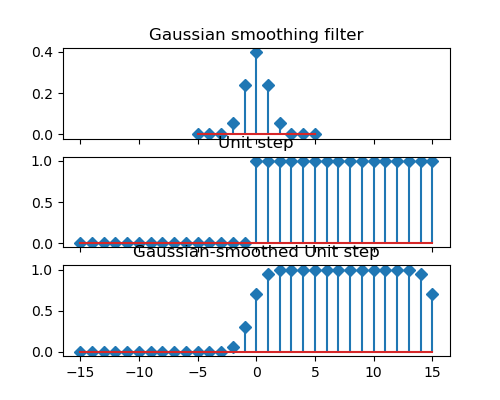
\includegraphics[height=2.5in]{mp3fig6.png}}
\end{frame}

%%%%%%%%%%%%%%%%%%%%%%%%%%%%%%%%%%%%%%%%%%%%
\section[Convolution]{Convolution}
\setcounter{subsection}{1}

\begin{frame}
  \frametitle{Convolution}
  \begin{itemize}
  \item A {\bf convolution} is exactly the same thing as a {\bf weighted local average}.
    We give it a special name, because we will use it very often.  It's defined as:
    \[
    y[n] = \sum_m g[m] f[n-m] = \sum_m g[n-m] f[m]
    \]
  \item 
    We use the symbol $\ast$ to mean ``convolution:''
    \[
    y[n]=g[n]\ast f[n] = \sum_m g[m] f[n-m] = \sum_m g[n-m] f[m]
    \]
  \end{itemize}
\end{frame}

\begin{frame}
  \frametitle{Convolution}
  \centerline{\fbox{$y[n] = g[n]\ast f[n] = \sum_m g[m] f[n-m] = \sum_m g[n-m] f[m]$}}

  \vspace*{2mm}
  
  Here is the pseudocode for convolution:
  \begin{enumerate}
  \item For every output $n$:
    \begin{enumerate}
    \item Reverse $g[m]$ in time, to create $g[-m]$.
    \item Shift it to the right by $n$ samples, to create $g[n-m]$.
    \item For every $m$:
      \begin{enumerate}
      \item Multiply $f[m]g[n-m]$.
      \end{enumerate}
    \item Add them up to create $y[n] = \sum_m g[n-m] f[m]$ for this particular $n$.
    \end{enumerate}
    \item Concatenate those samples together, in sequence, to make the signal $y$.
  \end{enumerate}
\end{frame}

\begin{frame}
  \frametitle{Convolution}
  \centerline{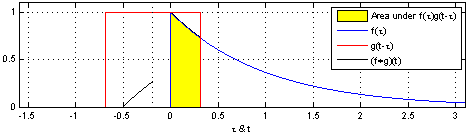
\includegraphics[width=\textwidth]{exp/convolution-94.png}}
  \begin{tiny}
    by Brian Amberg, CC-SA 3.0,
    \url{https://commons.wikimedia.org/wiki/File:Convolution_of_spiky_function_with_box2.gif}
  \end{tiny}
\end{frame}

\begin{frame}
  \frametitle{Convolution}
  \animategraphics[loop,controls,width=\linewidth]{20}{exp/convolution-}{0}{279}
  \begin{tiny}
    by Brian Amberg, CC-SA 3.0,
    \url{https://commons.wikimedia.org/wiki/File:Convolution_of_spiky_function_with_box2.gif}
  \end{tiny}
\end{frame}

\begin{frame}
  \frametitle{Convolution: how should you implement it?}
  Answer: use the numpy function, {\tt np.convolve}.  In general, if numpy has a function
  that solves your problem, you are {\em always} permitted to use it.

  \vspace*{2mm}
  
  \centerline{\fbox{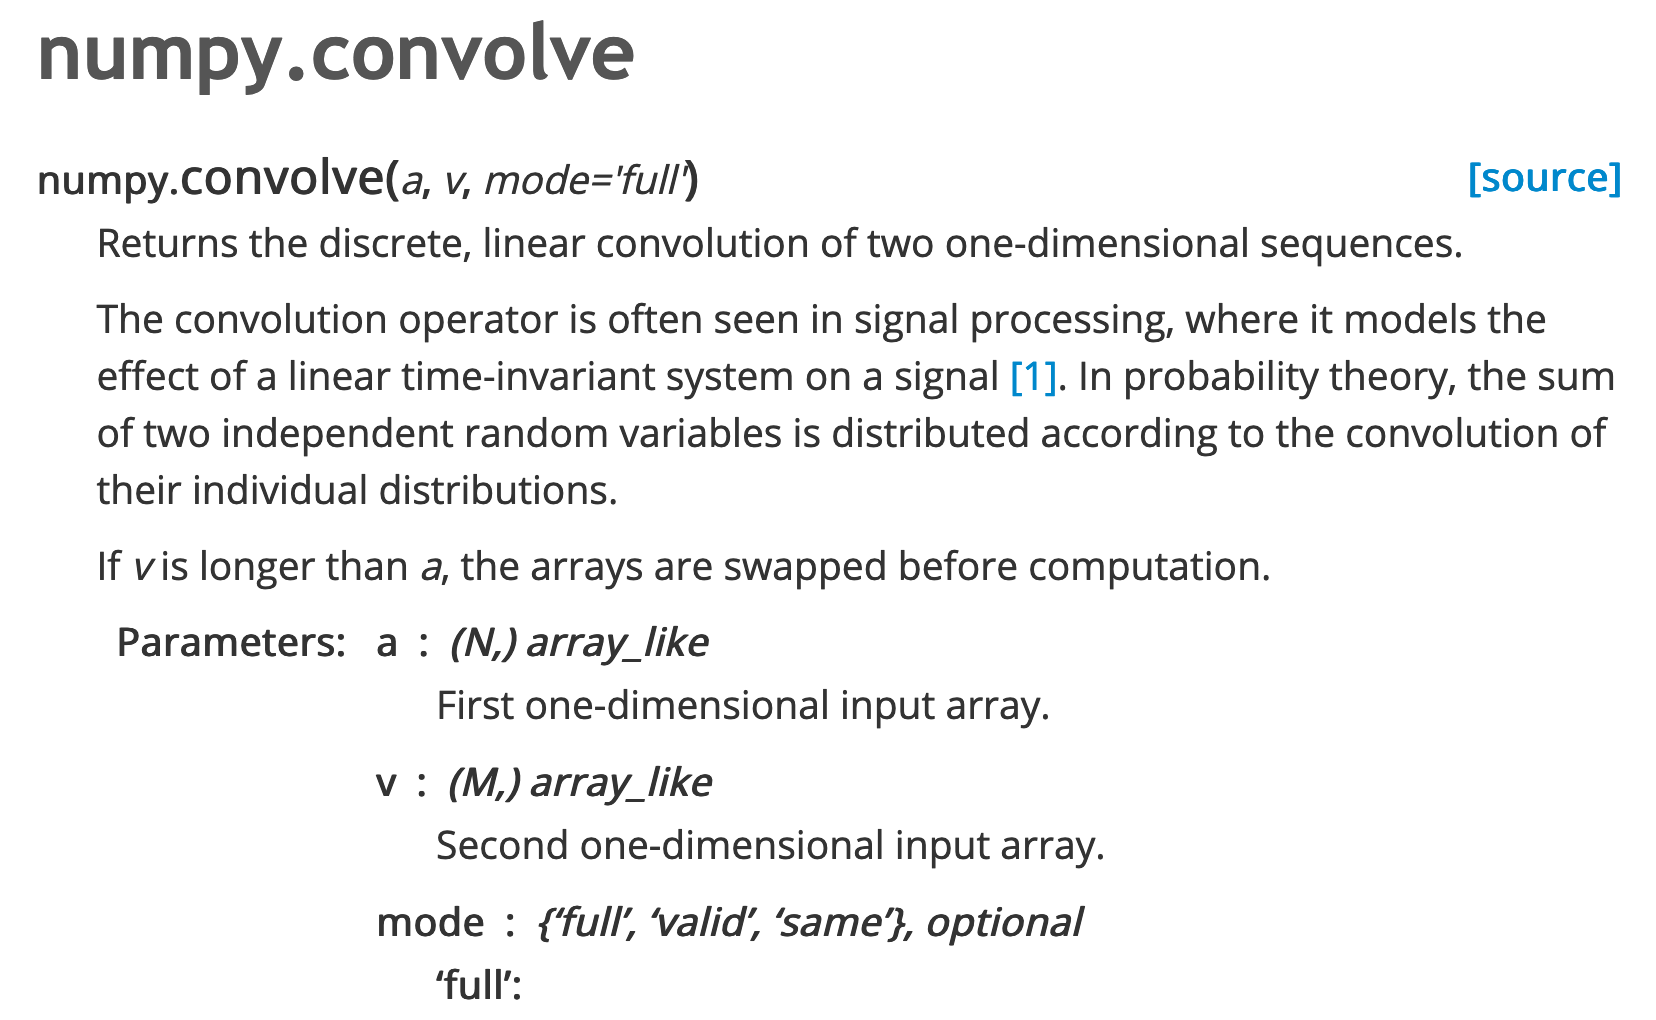
\includegraphics[height=2in]{numpy_convolve.png}}}
\end{frame}
  
%%%%%%%%%%%%%%%%%%%%%%%%%%%%%%%%%%%%%%%%%%%%
\section[Differencing]{Differencing}
\setcounter{subsection}{1}

\begin{frame}
  \frametitle{Differencing is convolution, too}

  Suppose we want to compute the local difference:
  \[
  y[n] = f[n] - f[n-1]
  \]
  We can do that using a convolution!
  \[
  y[n] = \sum_m f[n-m]h[m]
  \]
  where
  \[
  h[m] = \begin{cases}
    1 & m=0\\
    -1 & m=1\\
    0 & \mbox{otherwise}
  \end{cases}
  \]
\end{frame}

\begin{frame}
  \frametitle{Differencing as convolution} 
  \centerline{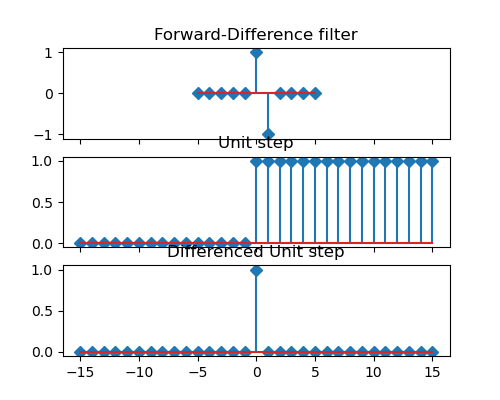
\includegraphics[height=2.5in]{mp3fig5.png}}
\end{frame}
  
%%%%%%%%%%%%%%%%%%%%%%%%%%%%%%%%%%%%%%%%%%%%
\section[Weighted]{Weighted Differencing}
\setcounter{subsection}{1}

\begin{frame}
  \frametitle{Weighted differencing as convolution}
  \begin{itemize}
    \item 
      The formula $y[n]=f[n]-f[n-1]$ is kind of noisy.  Any noise in
      $f[n]$ or $f[n-1]$ means noise in the output.
    \item
      We can make it less noisy  by
      \begin{enumerate}
      \item First, compute a weighted average:
        \[
        y[n] = \sum_m f[m]g[n-m]
        \]
      \item Then, compute a local difference:
        \[
        z[n] = y[n] - y[n-1] = \sum_m f[m]\left(g[n-m]-g[n-1-m]\right)
        \]
      \end{enumerate}
      This is exactly the same thing as convolving with
      \[
      h[n] = g[n]-g[n-1]
      \]
  \end{itemize}
\end{frame}

\begin{frame}
  \frametitle{A difference-of-Gaussians filter}

  The top row is a ``difference of Gaussians'' filter,
  $h[n]=g[n]-g[n-1]$, where $g[n]$ is a Gaussian.  The middle row is
  $f[n]$, the last row is the output $z[n]$.
  \centerline{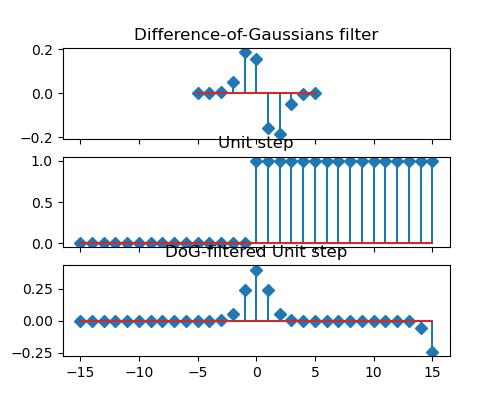
\includegraphics[height=2.5in]{mp3fig7.png}}
\end{frame}

\begin{frame}
  \frametitle{Difference-of-Gaussians filtering in both rows and columns}
      
  \centerline{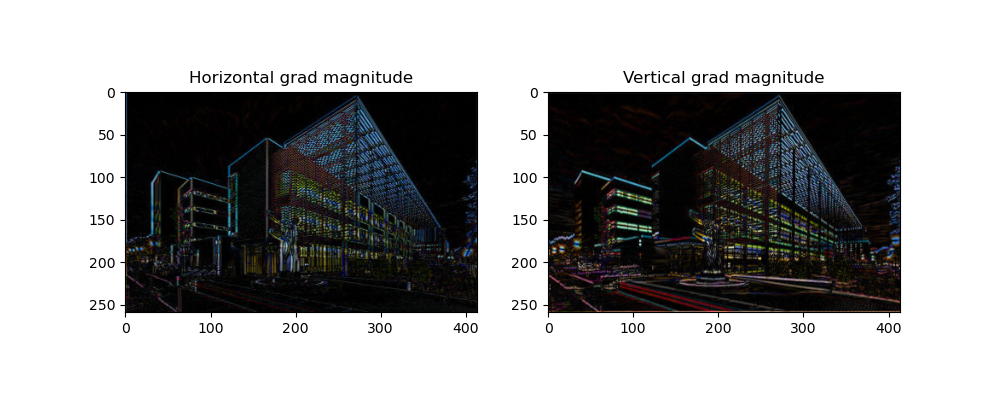
\includegraphics[height=2.5in]{mp3fig8.png}}
\end{frame}

%%%%%%%%%%%%%%%%%%%%%%%%%%%%%%%%%%%%%%%%%%%%
\section[Edges]{Edge Detection}
\setcounter{subsection}{1}

\begin{frame}
  \frametitle{Image gradient}
  \begin{itemize}
  \item Suppose we have an image $f[i,j,k]$.  The 2D image gradient is
    defined to be
    \[
    \vec{G}[i,j,k] = \left(\frac{df}{di}\right)\hat{i} + \left(\frac{df}{dj}\right)\hat{j}
    \]
    where $\hat{i}$ is a unit vector in the $i$ direction, $\hat{j}$
    is a unit vector in the $j$ direction.
  \item We can approximate these using the difference-of-Gaussians filter, $h_{dog}[n]$:
    \begin{align*}
      \frac{df}{di} &\approx G_i = h_{dog}[i]\ast f[i,j,k]\\
      \frac{df}{dj} &\approx G_j = h_{dog}[j]\ast f[i,j,k]\\
    \end{align*}
  \end{itemize}
\end{frame}
\begin{frame}
  \frametitle{The gradient is a vector}
  The image gradient, at any given pixel, is a vector.  It  points in the direction of
  increasing intensity (this image shows ``dark'' = greater intensity).
  \centerline{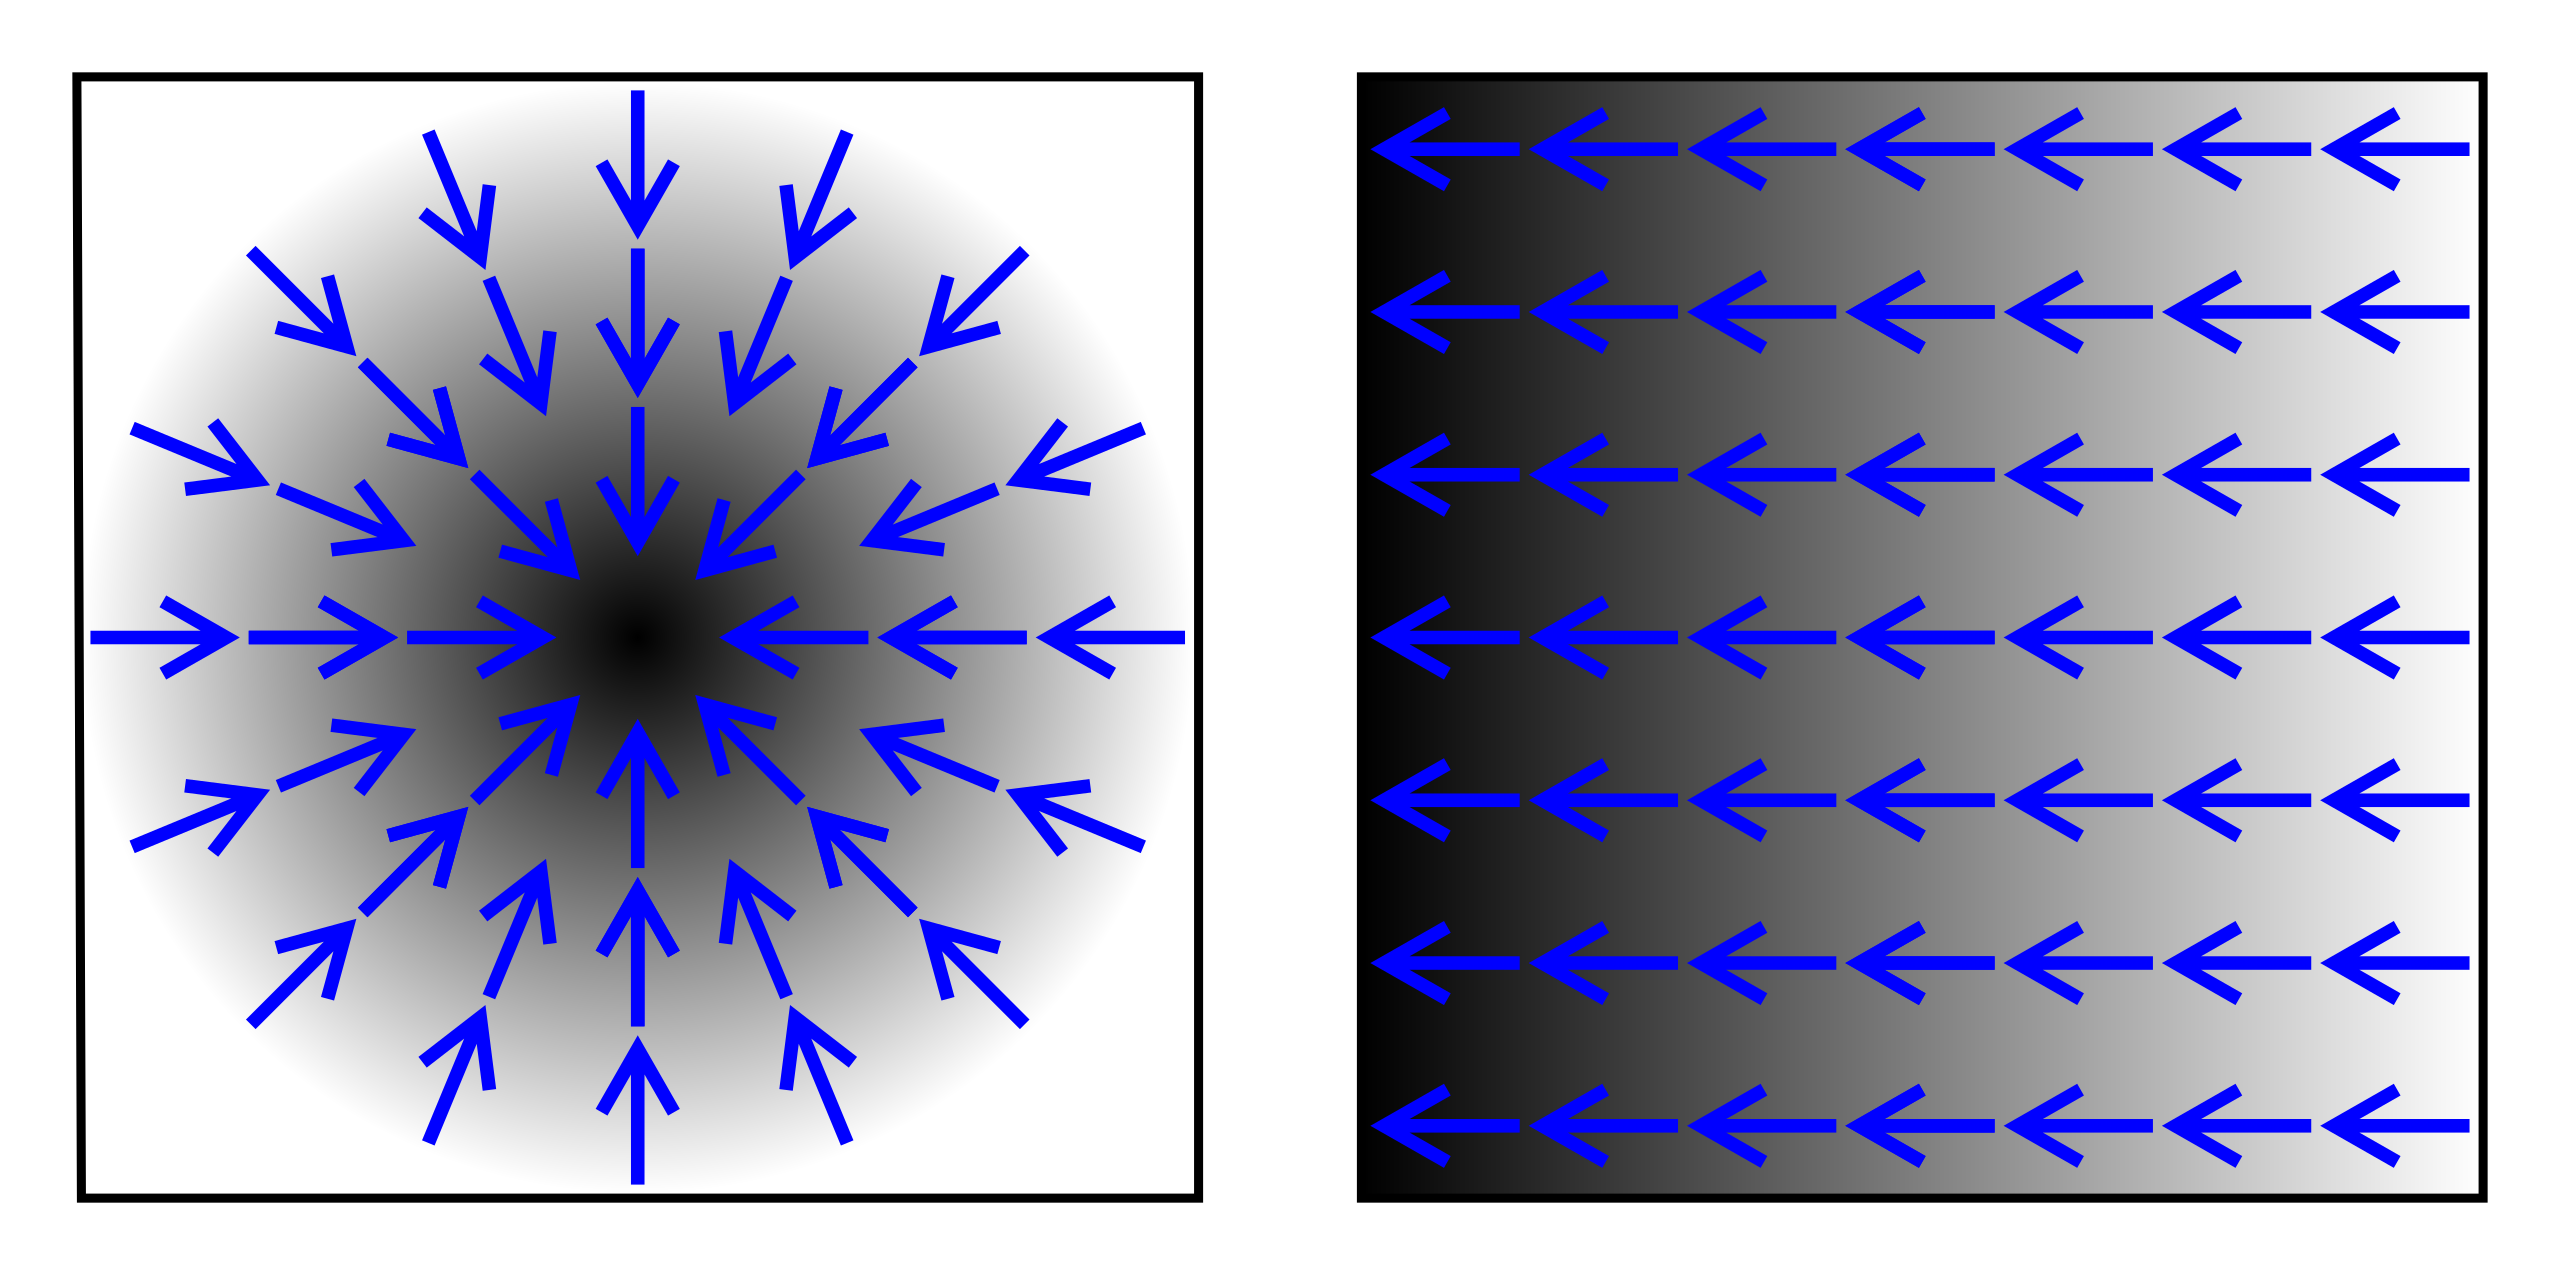
\includegraphics[height=2in]{exp/gradient.png}}
  \begin{tiny}
    By CWeiske, CC-SA 2.5,
    \url{https://commons.wikimedia.org/wiki/File:Gradient2.svg}
  \end{tiny}
\end{frame}
      
\begin{frame}
  \frametitle{Magnitude of the image gradient}
  \begin{itemize}
  \item
    The image gradient, at any given pixel, is a vector.
  \item
    It points in the direction in which intensity is increasing.
  \item
    The magnitude of the vector tells you how fast intensity is
    changing.
    \[
    \Vert \vec{G}\Vert =\sqrt{G_i^2 + G_j^2}
    \]
  \end{itemize}
\end{frame}
    
\begin{frame}
  \frametitle{Magnitude of the gradient = edge detector}
      
  \centerline{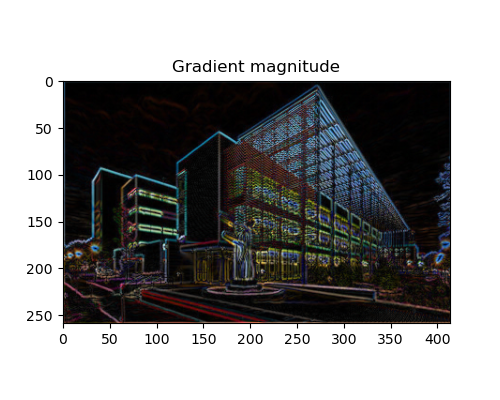
\includegraphics[height=3.5in]{mp3fig9.png}}
\end{frame}

%%%%%%%%%%%%%%%%%%%%%%%%%%%%%%%%%%%%%%%%%%%%
\section[Summary]{Summary}
\setcounter{subsection}{1}
\begin{frame}
  \frametitle{Summary}

    \[
    y[n] = g[n]\ast f[n] = \sum_m g[m] f[n-m] = \sum_m g[n-m] f[m]
    \]
\end{frame}

\end{document}
